%----------------------------------------------------------------------------------------
%	PACKAGES AND THEMES
%----------------------------------------------------------------------------------------
\documentclass[aspectratio=169,xcolor=dvipsnames]{beamer}
\usetheme{Simple}

\usepackage{hyperref}
\usepackage[russian]{babel}
\usepackage{graphicx} % Allows including images
\usepackage{booktabs} % Allows the use of \toprule, \midrule and \bottomrule in tables

%----------------------------------------------------------------------------------------
%	TITLE PAGE
%----------------------------------------------------------------------------------------

% The title
\title[short title]{Switch Transformers}

\author[Pin-Yen] {Илья Федоров, 417 группа}
\institute[NTU] % Your institution may be shorthand to save space
{
    % Your institution for the title page
    Факультет вычислительной математики и кибернетики \\
    МГУ им. М.В.Ломоносова
    \vskip 3pt
}
\date{\today} % Date, can be changed to a custom date


%----------------------------------------------------------------------------------------
%	PRESENTATION SLIDES
%----------------------------------------------------------------------------------------

\begin{document}

\begin{frame}
    % Print the title page as the first slide
    \titlepage
\end{frame}

\begin{frame}{Содержание}
    % Throughout your presentation, if you choose to use \section{} and \subsection{} commands, these will automatically be printed on this slide as an overview of your presentation
    \tableofcontents
\end{frame}

%------------------------------------------------
\section{Напоминание о трансформере}

%------------------------------------------------

\begin{frame}{Напоминание о трансформере}
\begin{center}
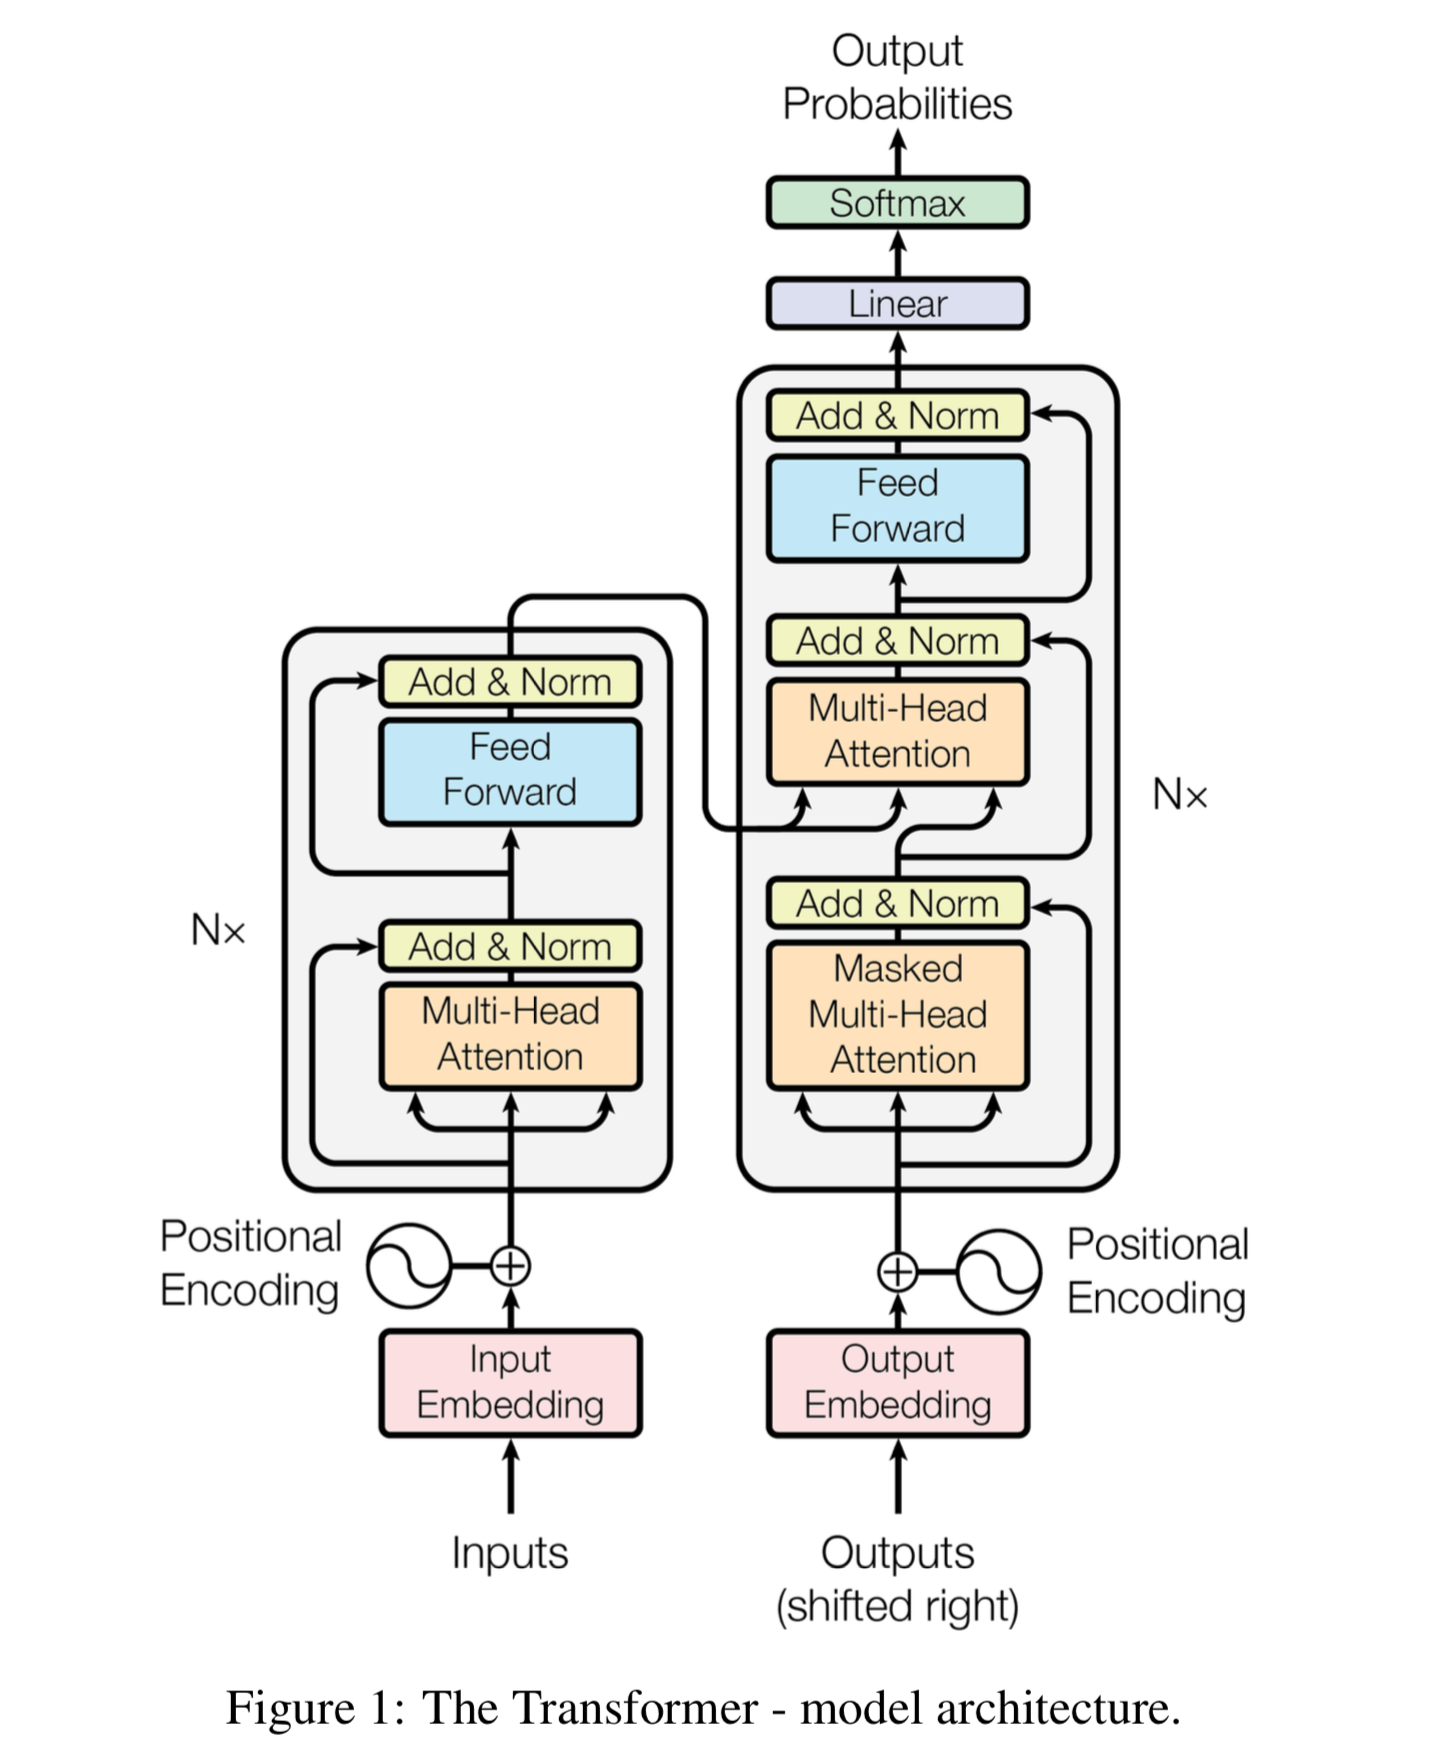
\includegraphics[scale=0.1]{trans.png}
Attention Is All You Need, Vaswani et al. 2017
\end{center}

\end{frame}

%------------------------------------------------
\section{Модель T5}

\begin{frame}{Модель T5}


\begin{figure}
\hspace{-7cm}
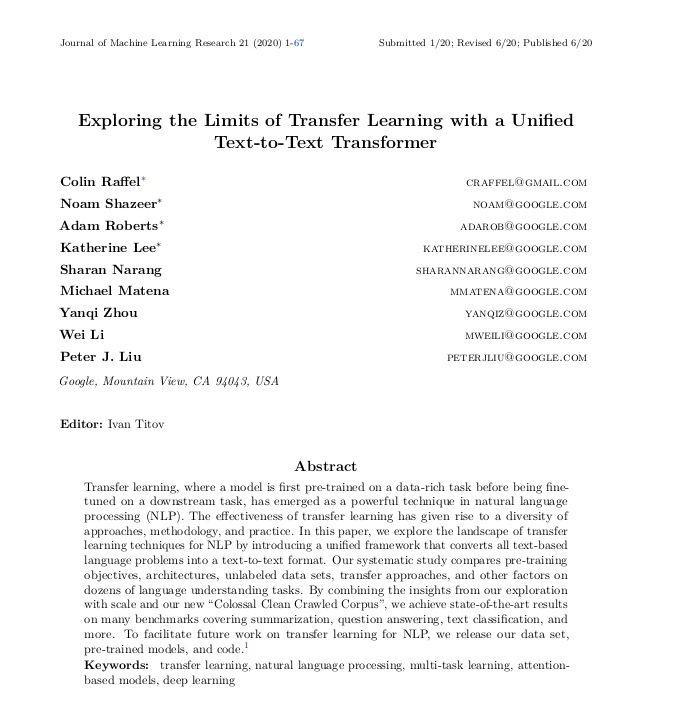
\includegraphics[scale=0.3]{t5.jpg}
\end{figure}

\begin{figure}
\vspace*{-5cm}
\hspace*{7cm}

\includegraphics[scale=0.6 ]{t52.jpg}
\end{figure}

\begin{center}
    
\end{center}



\end{frame}

\begin{frame}{Модель T5}
\begin{figure}
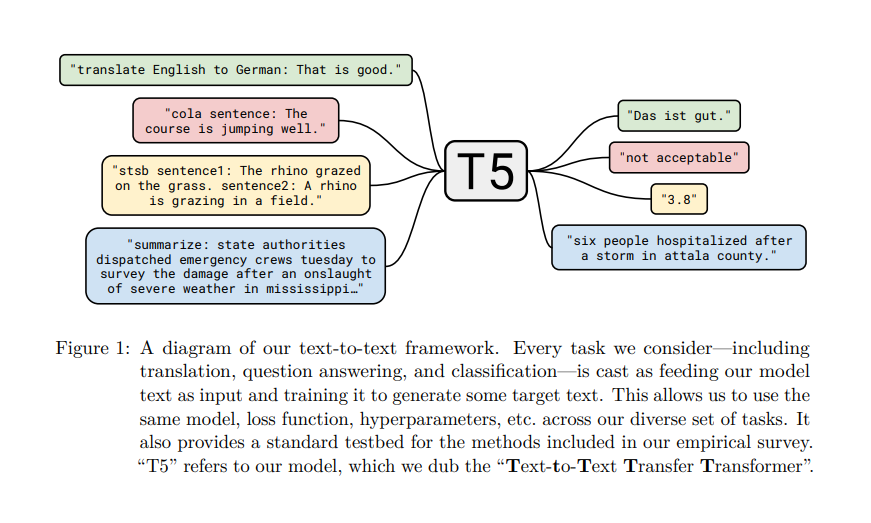
\includegraphics[scale=0.5]{11.png}
\end{figure}
\end{frame}

\begin{frame}{Модель T5}
\begin{figure}
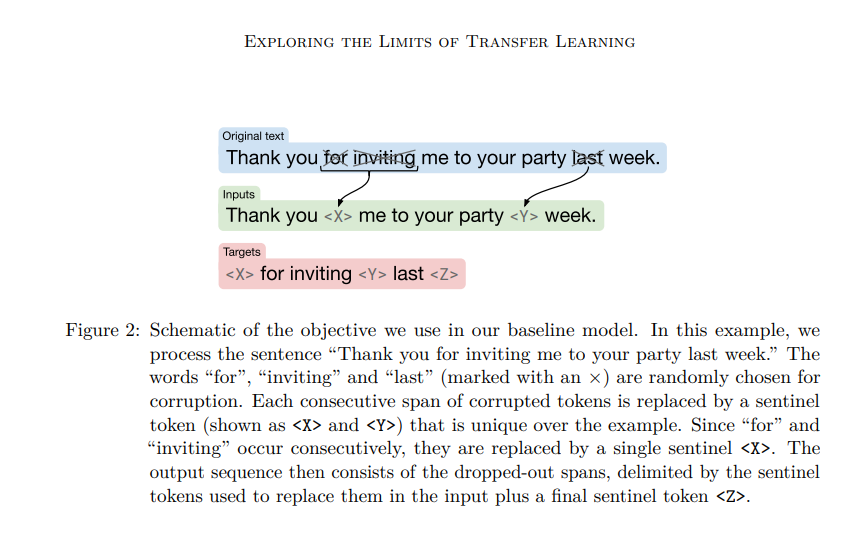
\includegraphics[scale=0.5]{12.png}
\end{figure}
\end{frame}

\begin{frame}{Модель T5}
\begin{figure}
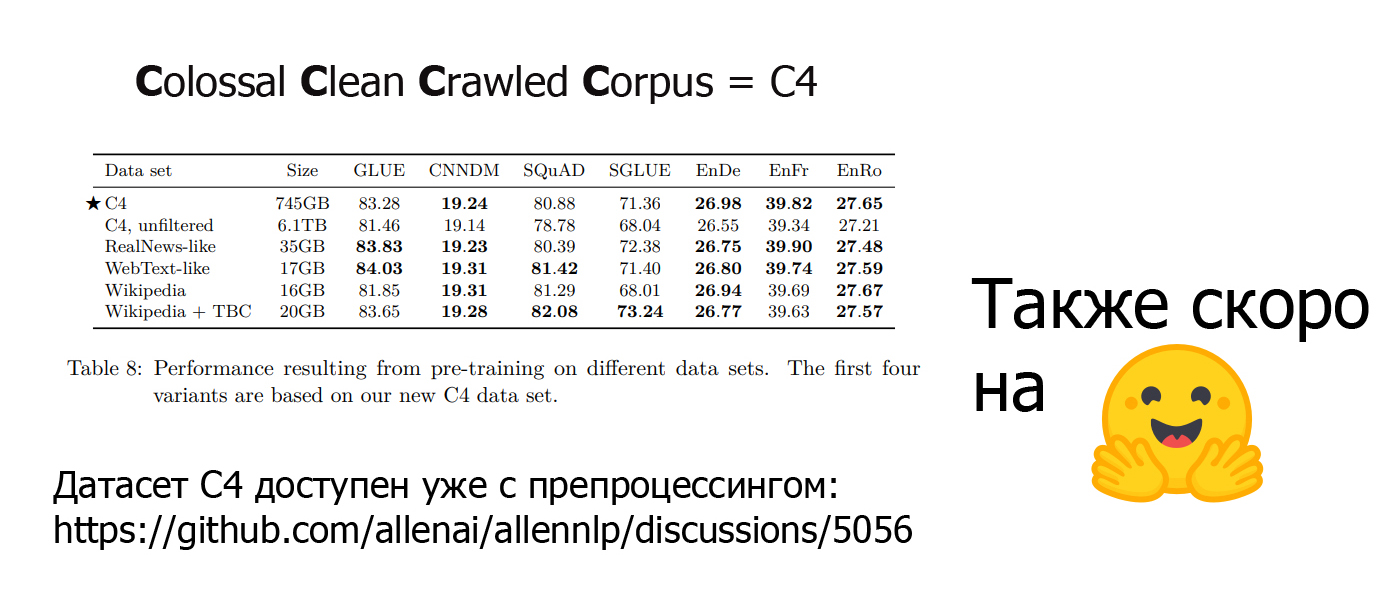
\includegraphics[scale=0.4]{kek.jpg}
\end{figure}

\end{frame}

\section{Switch Transformers}

\begin{frame}{Switch Transformers}
\begin{center}
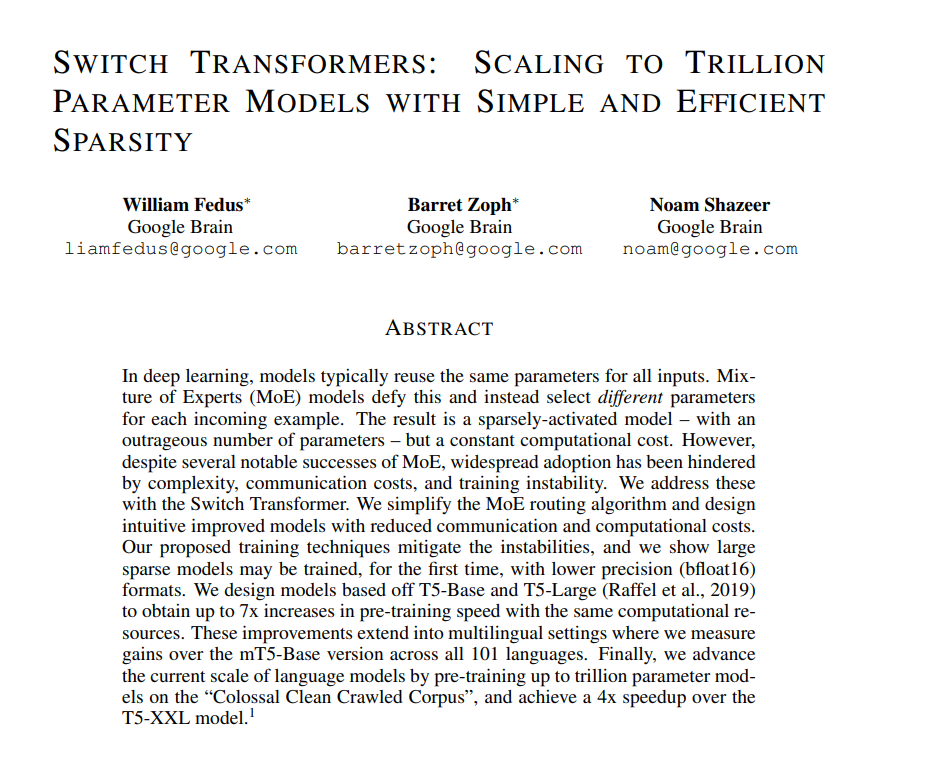
\includegraphics[scale=0.35]{switch1.png}    
\end{center} 
\end{frame}


\begin{frame}{Switch Transformers}
\begin{center}
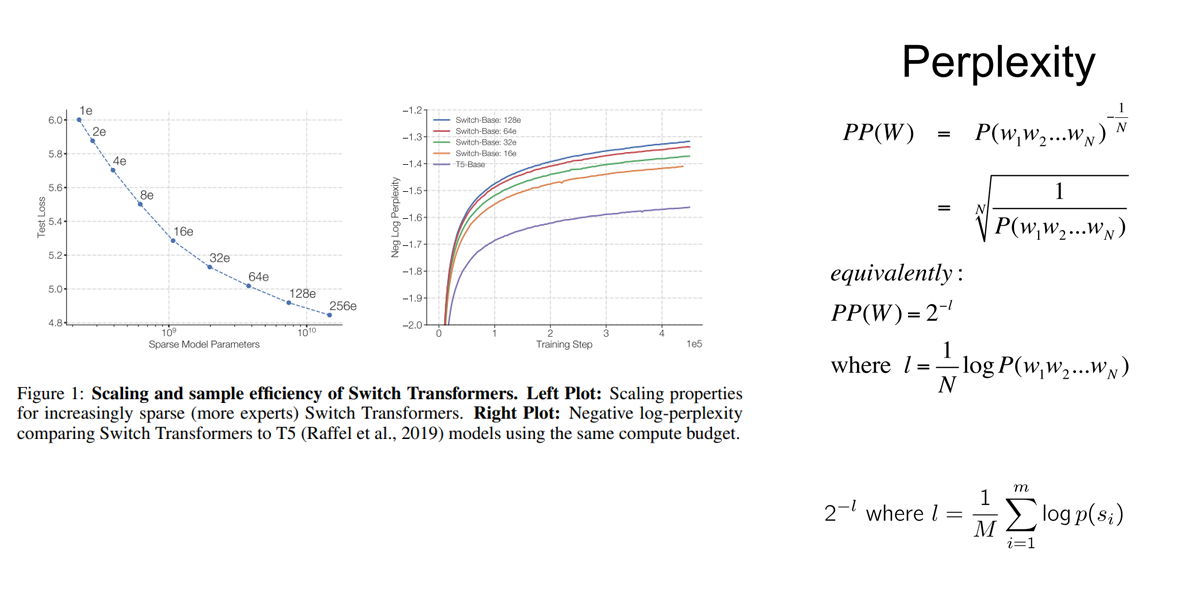
\includegraphics[scale=0.35]{switch2.png}    
\end{center} 
\end{frame}

\begin{frame}{Switch Transformers}
\begin{center}
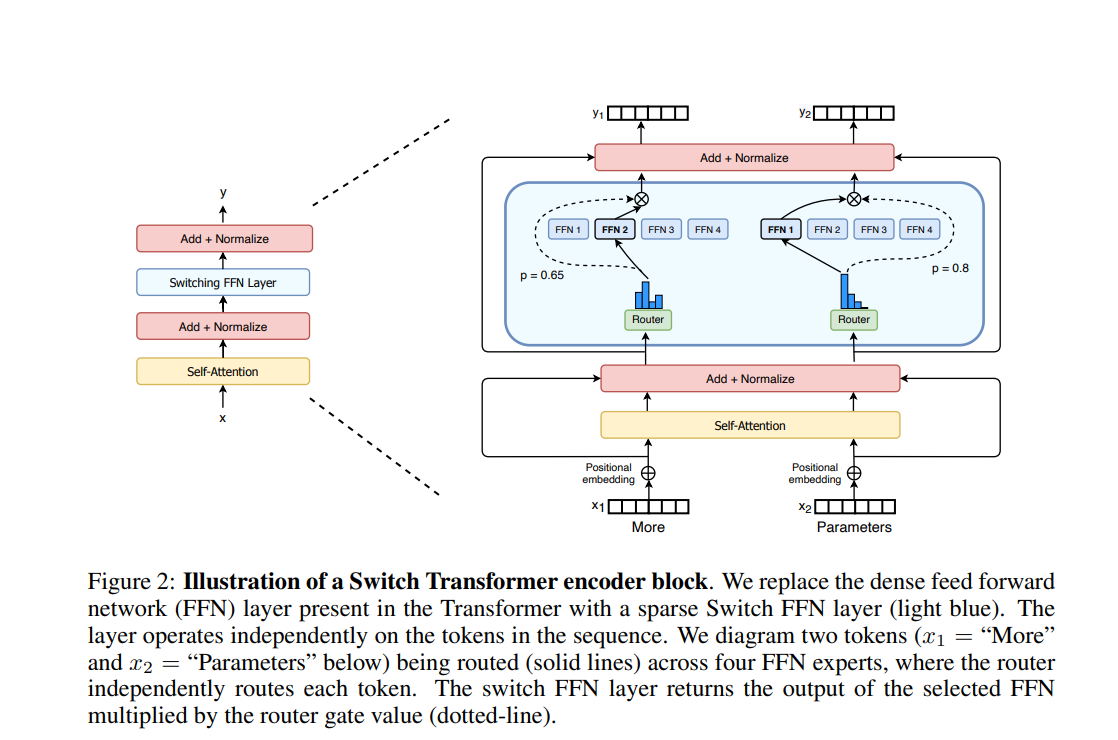
\includegraphics[scale=0.35]{switch3.png}    
\end{center} 
\end{frame}

\begin{frame}{Switch Transformers}
\begin{center}
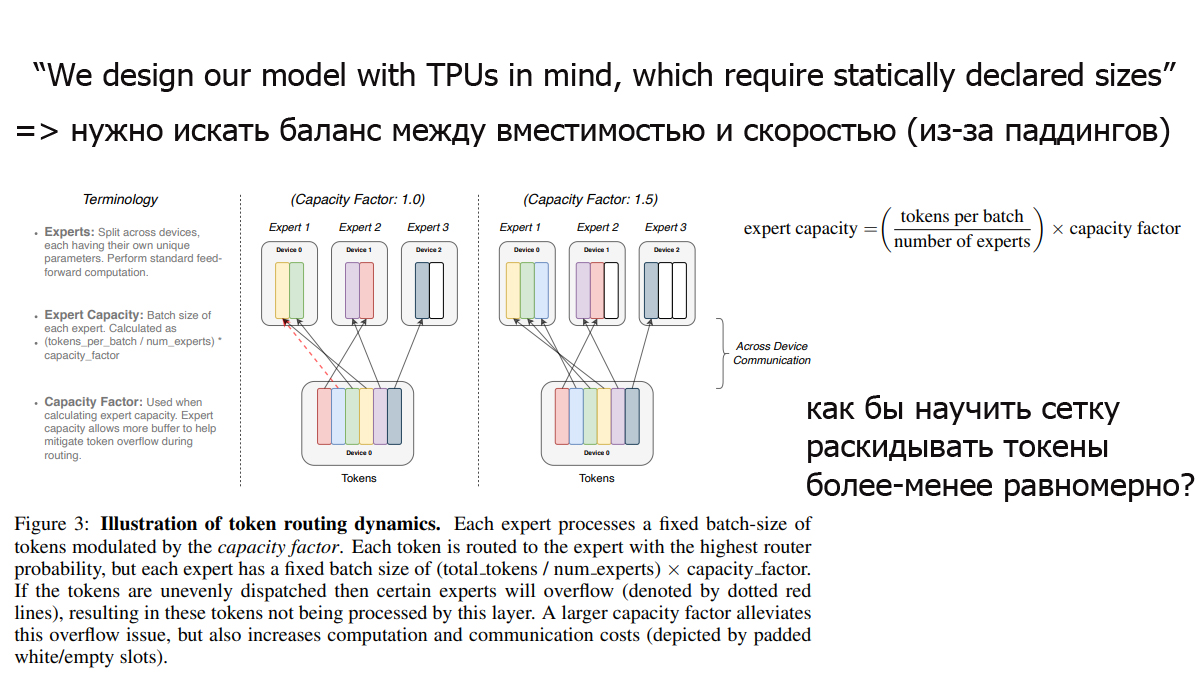
\includegraphics[scale=0.4]{st1.jpg}    
\end{center} 
\end{frame}

\begin{frame}{Switch Transformers}
\begin{center}
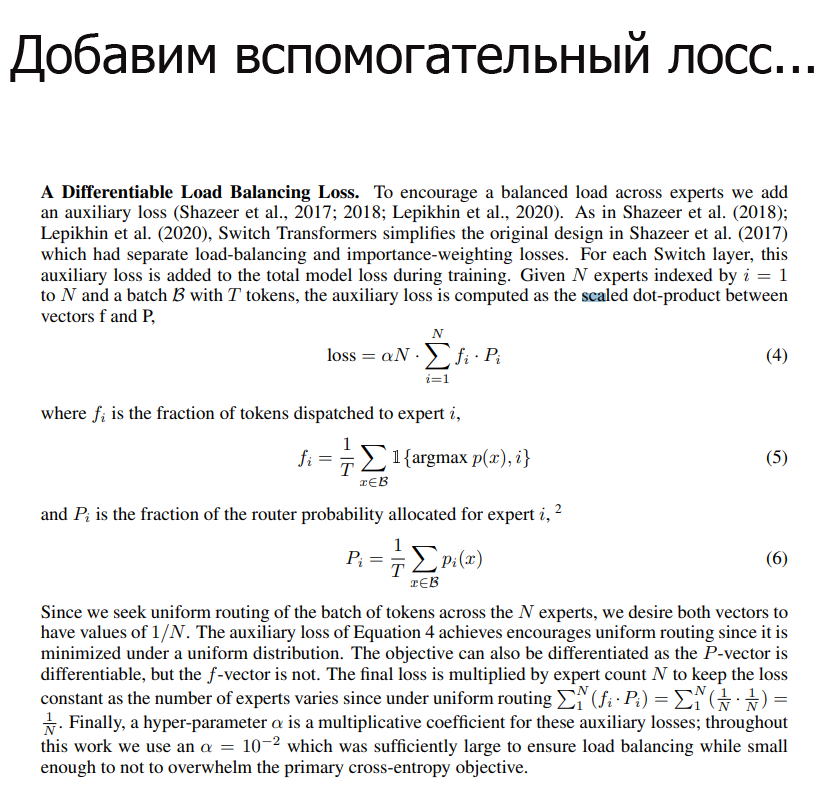
\includegraphics[scale=0.35]{st2.png}    
\end{center} 
\end{frame}

\begin{frame}{Switch Transformers}
\begin{center}
\vspace*{-0.5cm}
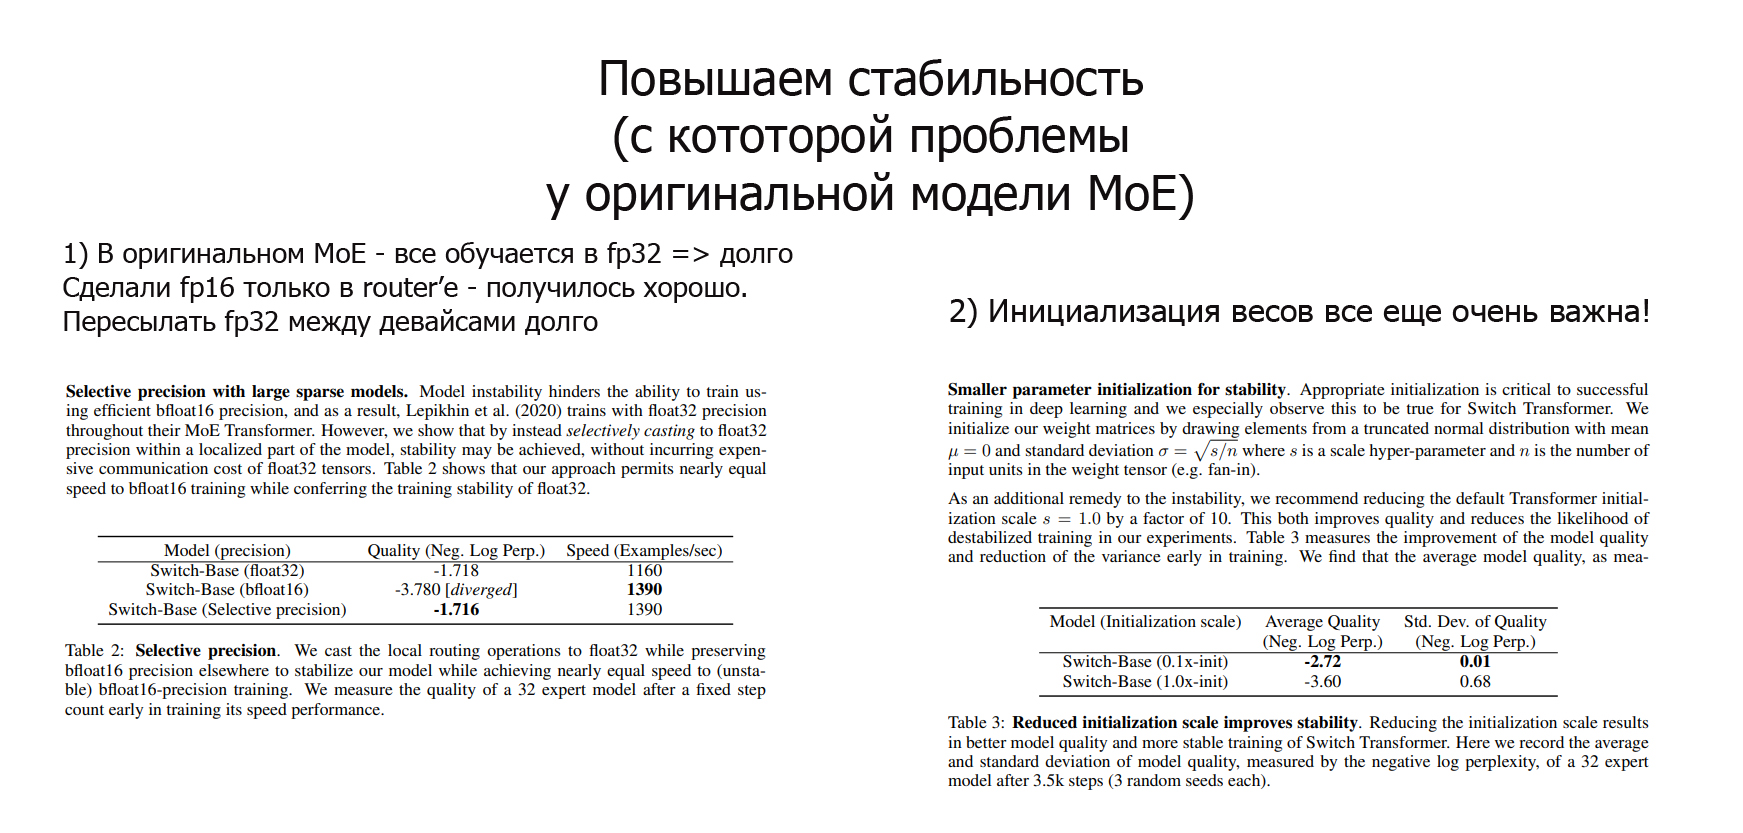
\includegraphics[scale=0.25]{st3.jpg}    
\end{center} 
\end{frame}

\begin{frame}{Switch Transformers}
\begin{center}
\vspace*{-0.5cm}
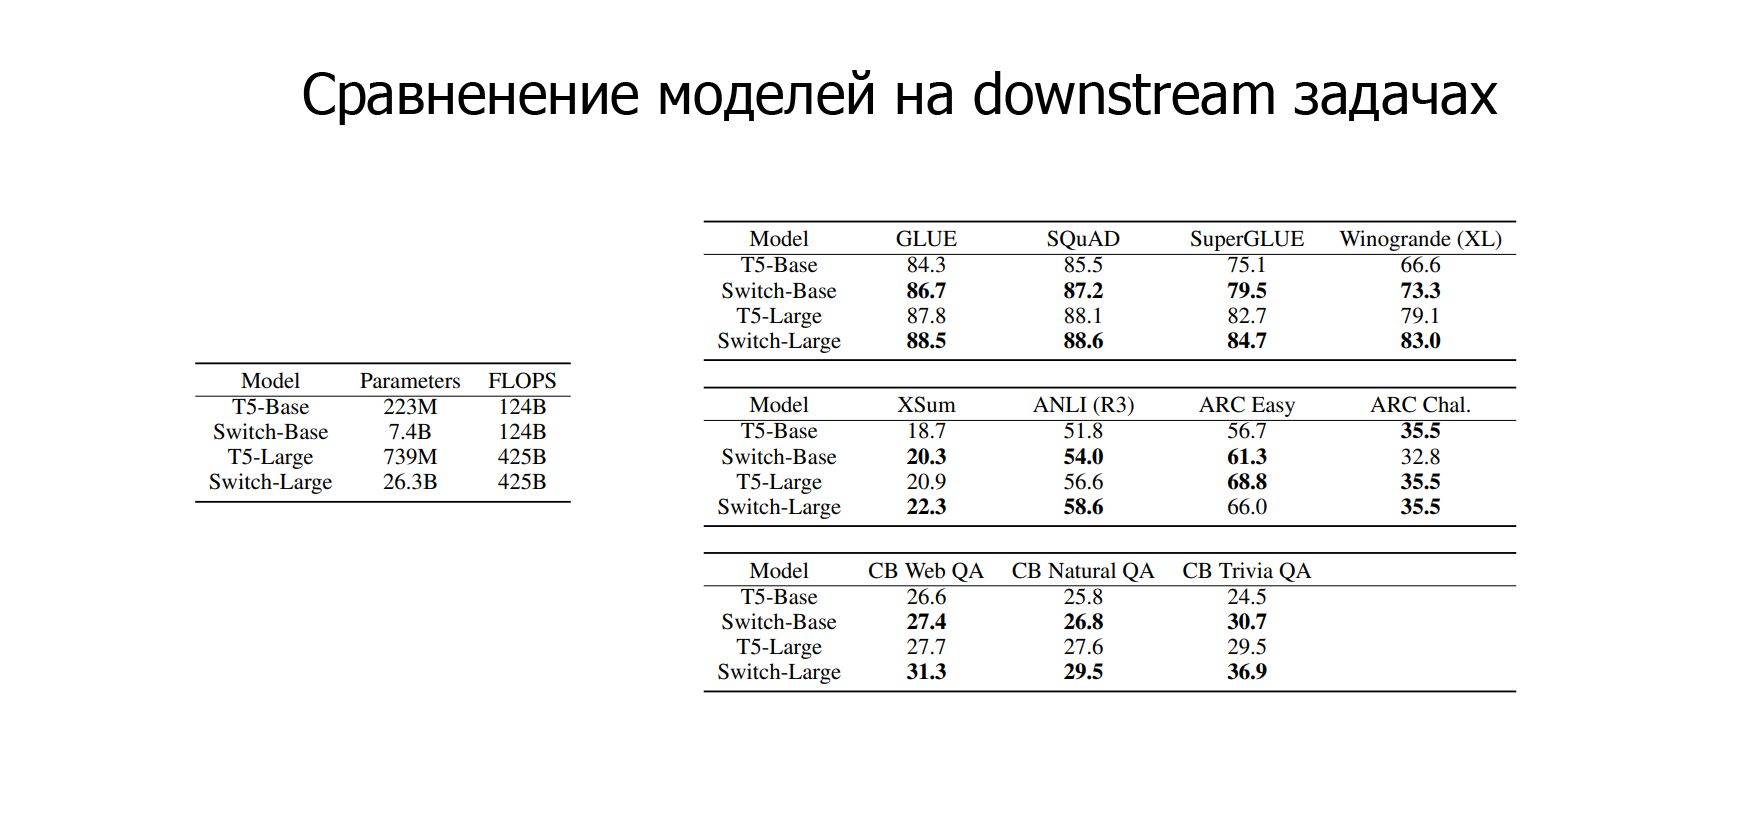
\includegraphics[scale=0.25]{st4.jpg}    
\end{center} 
\end{frame}

\begin{frame}{Switch Transformers}
\begin{center}
\vspace*{-0.5cm}
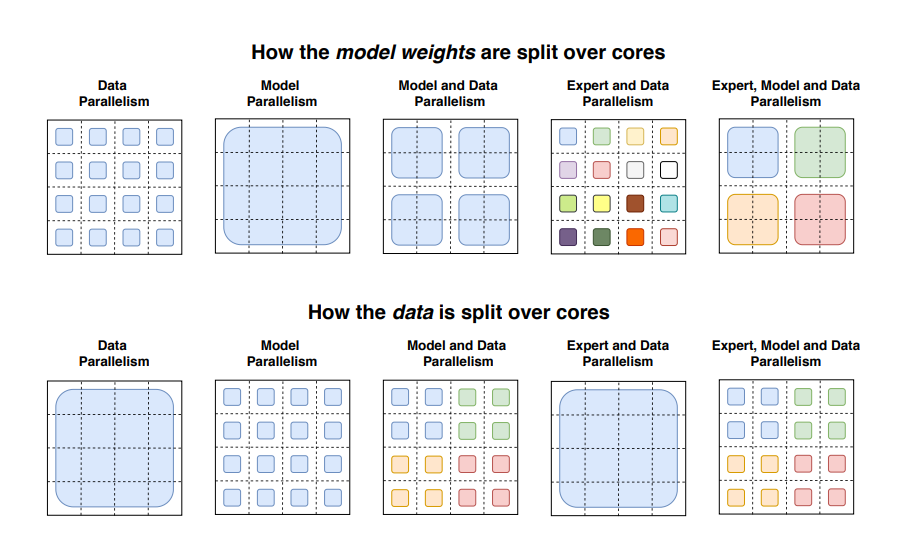
\includegraphics[scale=0.5]{st5.png}    
\end{center} 
\end{frame}

\begin{frame}{Switch Transformers}
\begin{center}
\vspace*{-0.5cm}
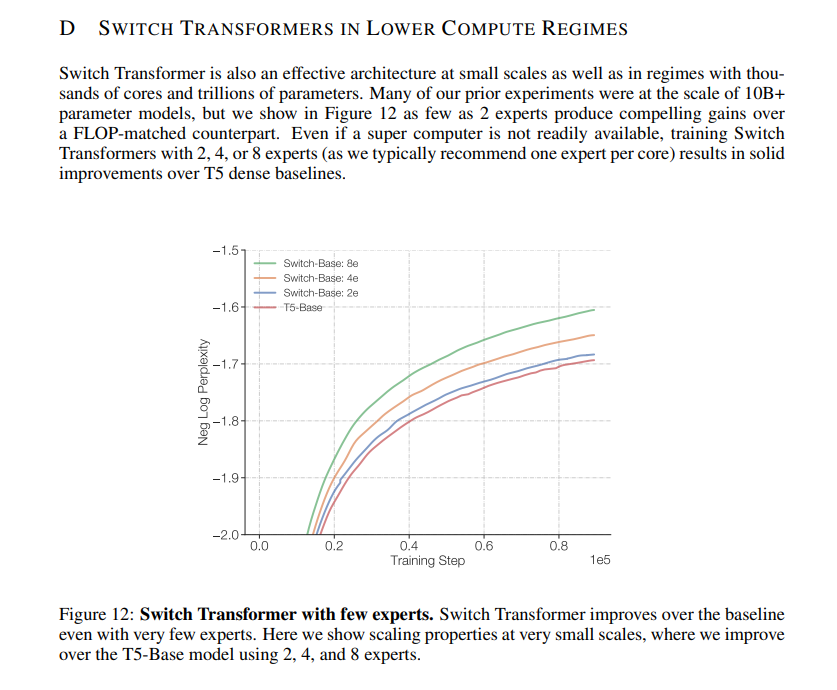
\includegraphics[scale=0.3]{st6.png}    
\end{center} 
\end{frame}

\end{document}